% !TEX encoding = UTF-8
% !TEX TS-program = pdflatex
% !TEX root = ../tesi.tex

%**************************************************************
\chapter{Progettazione e codifica}
\label{cap5}
%**************************************************************

\section{Design dell'interfaccia grafica}
\label{sec:design-gui}
Per definire un primo design dell'interfaccia grafica sono stati realizzati alcuni \gls{mock up}, utili anche per semplificare la progettazione e l'analisi dei vari aspetti relativi all'esperienza dell'utente.
Come da requisiti, l'interfaccia è stata sviluppata in modalità "wizard", ovvero una procedura a fasi dove l'utente deve completare l'azione richiesta da una fase per poter passare alla successiva.

Sono state individuate 3 fasi differenti (a cui corrispondono 3 pagine nell'interfaccia grafica), di seguito definite:

\begin{itemize}
\item La fase di \textit{training}: corrisponde alla prima fase, in cui viene creato il process model tramite tecniche di Machine Learning. Viene utilizzato l'event log caricato dall'utente contenente tracce complete (processi già terminati). L'utente potrà procedere alla fase successiva solo se il process model viene generato con successo;

\item La fase di \textit{runtime}: corrisponde alla seconda fase, in cui vengono generate le raccomandazioni. Viene utilizzato l'event log caricato dall'utente contenente tracce incomplete (processi ancora da terminare). L'utente potrà procedere solo se il processo di generazione delle raccomandazioni termina con successo;

\item La fase di visualizzazione: corrisponde alla terza ed ultima fase, in cui l'utente può visualizzare le raccomandazioni generate e le corrispettive spiegazioni. Questa fase rappresenta l'obiettivo finale dell'interfaccia, e la più "interessante" dal punto di vista dell'utente, che ha eseguito le fasi precedenti con lo scopo di visualizzare le raccomandazione e spiegazioni a cui era interessato.

\end{itemize}

Con il termine \textbf{esperimento} ci si riferirà, nel resto del testo, ad una singola esecuzione completa di almeno la prima fase.

\subsection{Fase di training}
\label{subsec:training-phase}

\begin{figure}[H] 
    \centering 
    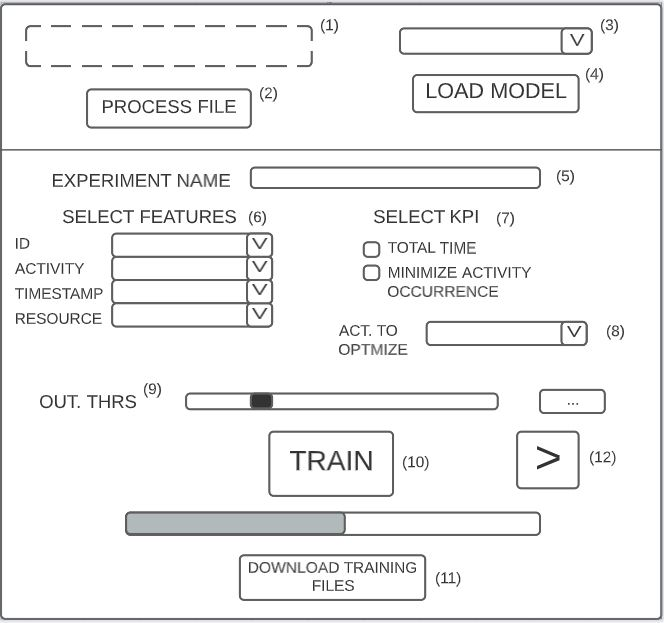
\includegraphics[width=0.9\columnwidth]{immagini/mockup-train.jpg} 
    \caption{Design iniziale della pagina relativa alla fase di training}
    \label{fig:mockup-train}
\end{figure}

In \autoref{fig:mockup-train} il mock up su cui si è basato l'aspetto finale della pagina relativa alla fase di training.
\\
Seguendo i requisiti, il flusso principale di utilizzo della pagina è il seguente (i riferimenti numerici successivi, in forma (x), sono relativi alla \autoref{fig:mockup-train}):

\begin{enumerate}
\item L'utente carica l'event log che vuole utilizzare per il processo di training, usando l'area di \gls{drag-and-drop} (1) e clicca il pulsante "Process file" (2) che permette all'interfaccia di analizzare ed elaborare il file caricato;

\item L'utente dichiara i nomi delle colonne dell'event log caricato, corrispondenti alle features richieste, usando gli elementi \gls{dropdown} (6), le opzioni disponibili sono l'insieme delle colonne dell'event log caricato (grazie alla fase di elaborazione). Questo semplifica e velocizza il processo di compilazione, in quanto l'utente deve solo selezionare la colonna giusta al posto di scriverla, riducendo gli errori. Da notare come le features sono tutte obbligatorie tranne la feature "resource";

\item L'utente seleziona il KPI che desidera (7), se sceglie "Minimize activity occurrence" dovrà anche dichiarare il nome dell'attività da ottimizzare, tramite l'apposito \gls{dropdown} (8), che anche qui semplifica e velocizza la compilazione in quanto contiene già l'insieme di tutte le attività presenti nell'event log;

\item L'utente inserisce il nome dell'esperimento nella casella di testo (5) apposita e seleziona, tramite uno \gls{slider} (9), la soglia degli outliers che desidera (essa ha comunque un valore di default iniziale);

\item L'utente avvia il processo di training cliccando sul pulsante "Train" (10);

\item Al termine del processo di training l'utente può, se lo desidera, scaricare i file che compongono il process model cliccando il pulsante "Download training files" (11); 

\item Infine l'utente può passare alla pagina successiva cliccando sul pulsante a freccia (12).

\end{enumerate}

Va evidenziato che lo step 4. può essere effettuato in qualsiasi momento, basta che sia prima del passo 5. e dopo il passo 1., mentre il passo 6. è opzionale. 
\\ \\
Se è già presente un process model (creato in un esperimento precedente) è possibile caricarlo nel sistema e saltare tutto il processo di training (che può richiedere una quantità di tempo considerevole). Il flusso di esecuzione alternativo è il seguente (i riferimenti numerici successivi, in forma (x), sono relativi alla \autoref{fig:mockup-train}):

\begin{enumerate}
\item L'utente seleziona un process model già creato tra quelli disponibili, usando l'apposito \gls{dropdown} (3) e clicca il pulsante "Load model" (4) per caricare il process model nel sistema;

\item L'utente può, se lo desidera, scaricare i file che compongono il process model cliccando il pulsante "Download training files" (11); 

\item Infine l'utente può passare alla pagina successiva cliccando sul pulsante a freccia (12).

\end{enumerate}

In questo caso invece, il passo 2. è da considerarsi opzionale.


\subsection{Fase di runtime}
\label{subsec:training}

\begin{figure}[!h] 
    \centering 
    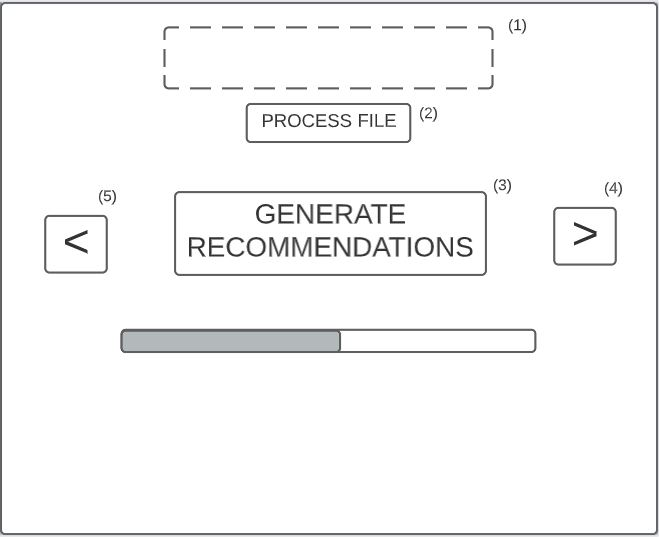
\includegraphics[width=0.8\columnwidth]{immagini/mockup-run.jpg} 
    \caption{Design iniziale della pagina relativa alla fase di runtime}
    \label{fig:mockup-run}
\end{figure}

In \autoref{fig:mockup-run} il mock up su cui si è basato l'aspetto finale della pagina relativa alla fase di runtime.
\\
Seguendo i requisiti, il flusso principale di utilizzo della pagina è il seguente (i riferimenti numerici successivi, in forma (x), sono relativi alla \autoref{fig:mockup-run}):

\begin{enumerate}

\item L'utente carica l'event log che vuole utilizzare per la generazione delle raccomandazioni, usando l'area di \gls{drag-and-drop} (1) e clicca il pulsante "Process file" (2) che permette all'interfaccia di analizzare ed elaborare il file caricato;

\item L'utente clicca sul pulsante "Generate recommendations" (3) per avviare il processo di generazione delle raccomandazioni;

\item Al termine del processo di generazione delle raccomandazioni l'utente può passare alla pagina successiva cliccando sul pulsante a freccia (4).

\end{enumerate}


\subsection{Fase di visualizzazione}

\begin{figure}[!h] 
    \centering 
    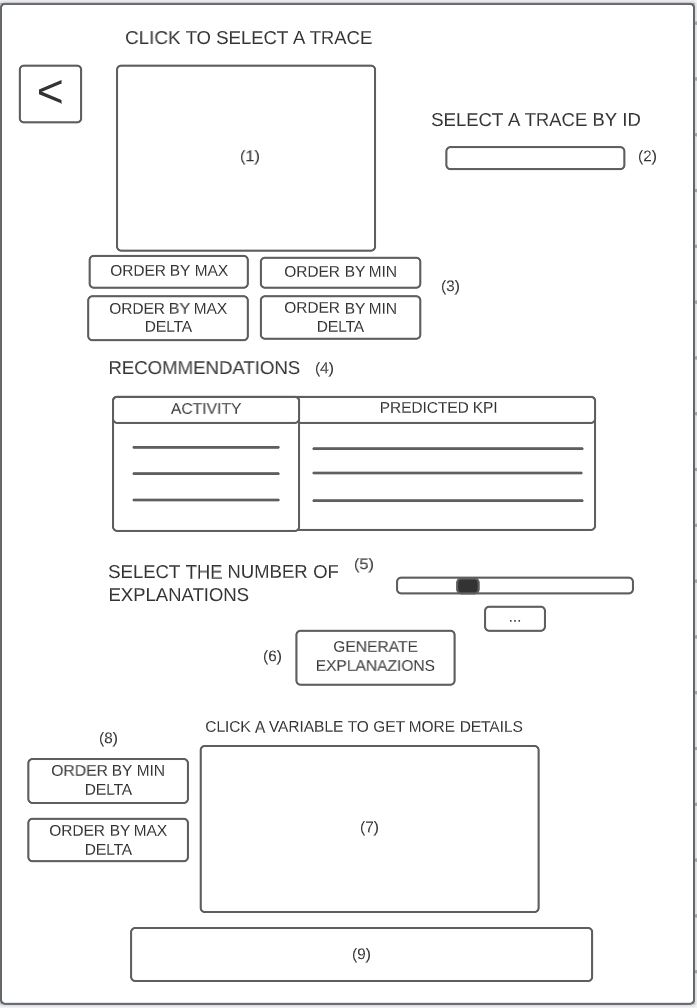
\includegraphics[width=0.7\columnwidth]{immagini/mockup-explain.jpg} 
    \caption{Design iniziale della pagina relativa alla fase di visualizzazione}
    \label{fig:mockup-explain}
\end{figure}

In \autoref{fig:mockup-explain} il mock up su cui si è basato l'aspetto finale della pagina relativa alla fase di visualizzazione.
\\
Seguendo i requisiti il flusso principale di utilizzo della pagina è il seguente (i riferimenti numerici successivi, in forma (x), sono relativi alla \autoref{fig:mockup-explain}):

\begin{enumerate}
\item L'utente visualizza, tramite il grafico (1), la migliore delle 3 raccomandazioni generate, e ha la possibilità di selezionare una traccia cliccando sulla rispettiva raccomandazione nel grafico oppure inserendo la traccia nella casella di testo apposita (2);

\item L'utente, se desidera, può riordinare le raccomandazioni generate usando uno dei 4 pulsanti in (3);

\item Una volta selezionata la traccia l'utente può visualizzare il resto delle raccomandazioni generate, con relativo KPI predetto nella tabella (4);

\item L'utente può selezionare una delle raccomandazioni di cui vuole visualizzare la spiegazione, tramite un click sulla corrispondente riga della tabella (4);

\item L'utente può scegliere la quantità di variabili da visualizzare nella spiegazione tramite lo \gls{slider} apposito (5), in ogni caso viene definita una quantità di default;

\item L'utente avvia il processo di generazione della spiegazione cliccando sul pulsante "Generate explanazions" (6);

\item Al termine del processo di generazione della spiegazione l'utente può visualizzarla nel grafico apposito (7);

\item L'utente, se desidera, può riordinare le variabili della spiegazione generata usando uno dei 2 pulsanti in (8);

\item L'utente può cliccare su una specifica variabile della spiegazione generata per ottenere maggiori dettagli in formato testuale nello spazio designato (9).

\end{enumerate}

Alcune osservazioni sui punti 1. e 3.: il sistema genera fino ad un massimo di 3 raccomandazioni per traccia, la scelta di visualizzare sul grafico solo la migliore delle 3, come descritto nel punto 1., era per evitare di saturare il grafico. Va considerato infatti, che l'utente sarà interessato maggiormente alla migliore delle raccomandazioni. Poi è libero di consultare il resto delle raccomandazioni generate ma in forma solo testuale, come descritto nel punto 3., un grafico troppo saturo avrebbe sono effetti negativi sulla comprensione dell'utente.


\section{Architettura del sistema}
L'architettura del sistema segue il \gls{design pattern} \textbf{MVP}, molto comune per lo sviluppo di interfacce grafiche. 


\begin{figure}[H] 
    \centering 
    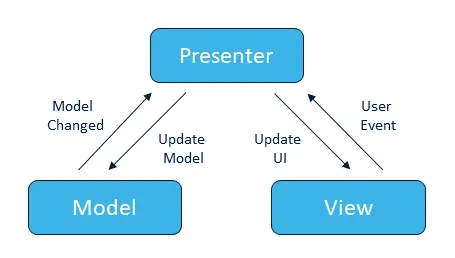
\includegraphics[width=0.9\columnwidth]{immagini/mvp.png} 
    \caption{Struttura design pattern MVP \cite{site:mvp}}
    \label{fig:mvp}
\end{figure}

Esso è composto da 3 componenti principali:

\begin{itemize}

\item \textit{Model}: Contiene la logica di business, ovvero i dati a cui siamo interessati, ed è responsabile della loro gestione (lettura, scrittura, modifica);

\item \textit{View}: Rappresenta l'interfaccia più a stretto contatto con l'utente e si occupa di mostrare i dati e di raccogliere l'input dell'utente. Nel caso particolare del MVP, la vista è passiva, quindi non dovrebbe contenere nessuna logica applicativa ma solo visuale;

\item \textit{Presenter}: Rappresenta il ponte do comunicazione tra View e Model, riceve gli input dalla View, si occupa di recuperare i dati e dell'esecuzione della logica di business da parte del Model, per poi formattare e inviare alla View i dati da visualizzare.

\end{itemize}

Un'aspetto importante è il fatto che la View non ha conoscenze (e nessuna dipendenza) dal Model e viceversa. 
\\
Questo porta ai principali motivi che hanno spinto a scegliere il \gls{design pattern}:

\begin{itemize}

\item Testabilità: le singole parti possono essere testate in isolamento più facilmente dato che le logiche applicative e visuali sono separate;

\item Separazione dei compiti: la separazione logiche e la ridotta dipendenza tra le parti (in particolare Model e View sono totalmente separati) permette di avere codice più modulare, quindi semplice e mantenibile;

\item Compatibilità con il framework: vista la forma dichiarativa delle viste costruite con il framework Dash si adatta bene alla View passiva caratteristica del MVP.

\end{itemize}

\section{Progettazione classi dell'interfaccia grafica}
Di seguito saranno utilizzati i digrammi \gls{UML} per la rappresentazione delle classi che compongono l'interfaccia.

\subsection{Progettazione View}
\label{subsec:prog-views}
Per la progettazione della componente View è stata sviluppata una struttura a views multiple, una per ogni pagina descritta nella \autoref{sec:design-gui}.

\begin{figure}[H] 
    \centering 
    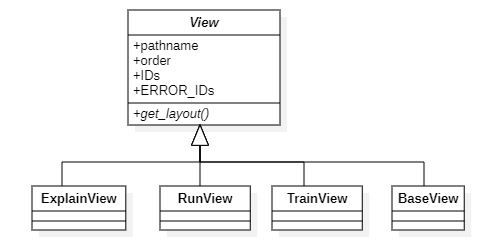
\includegraphics[width=0.8\columnwidth]{immagini/uml-views.jpg} 
    \caption{Diagramma UML per la classi della View}
    \label{fig:uml-views}
\end{figure}

Viene definita una classe astratta, che rappresenta una view generica, sulla quale si basano le altre views. Questo è utile per esporre le funzionalità comuni che deve avere una view.
In particolare ogni view deve definire:

\begin{itemize}

\item Un attributo \texttt{pathname} che rappresenta il nome della vista, usato per sviluppare l'interfaccia in modalità wizard;

\item Un attributo \texttt{order} che rappresenta l'ordimento utilizzato per mostrare le pagine, serve a definire i predecessori e/o successori di ogni pagina, usato per sviluppare l'interfaccia in modalità wizard;

\item Un attributo \texttt{IDs} che definisce l'insieme di tutti gli identificativi univoci dei componenti usati dal framework Dash per la costruzione della parte grafica dell'interfaccia; 

\item Un attributo \texttt{ERROR\_IDs} che definisce l'insieme di tutti gli identificativi univoci dei componenti usati dal framework Dash per visualizzare gli eventuali messaggi d'errore; 

\item L'implementazione del metodo astratto \texttt{get\_layout} che definisce il layout dell'applicazione web composto dall'insieme dei componenti Dash e la loro struttura, per la creazione della parte grafica della specifica pagina.

\end{itemize}

Sono state definite 4 classi concrete che implementano la classe \texttt{View}:
\begin{itemize}
\item La classe \texttt{TrainView} relativa alla pagina per la fase di training, 
\item La classe \texttt{RunView} relativa alla pagina per la fase di runtime, 
\item La classe \texttt{ExplainView} relativa alla pagina per la fase di visualizzazione;
\item La classe \texttt{BaseView} che si occupa della gestione dei componenti comuni a tutte le view (ad esempio i pulsanti per navigare tra le pagine).
\end{itemize}


\subsection{Progettazione Model}
\label{subsec:prog-model}
La progettazione del Model ha tenuto conto del back-end sottostante, cercando di suddividere la struttura in classi specializzate, promuovendo l'incapsulamento e la modularità.

\begin{figure}[H] 
    \centering 
    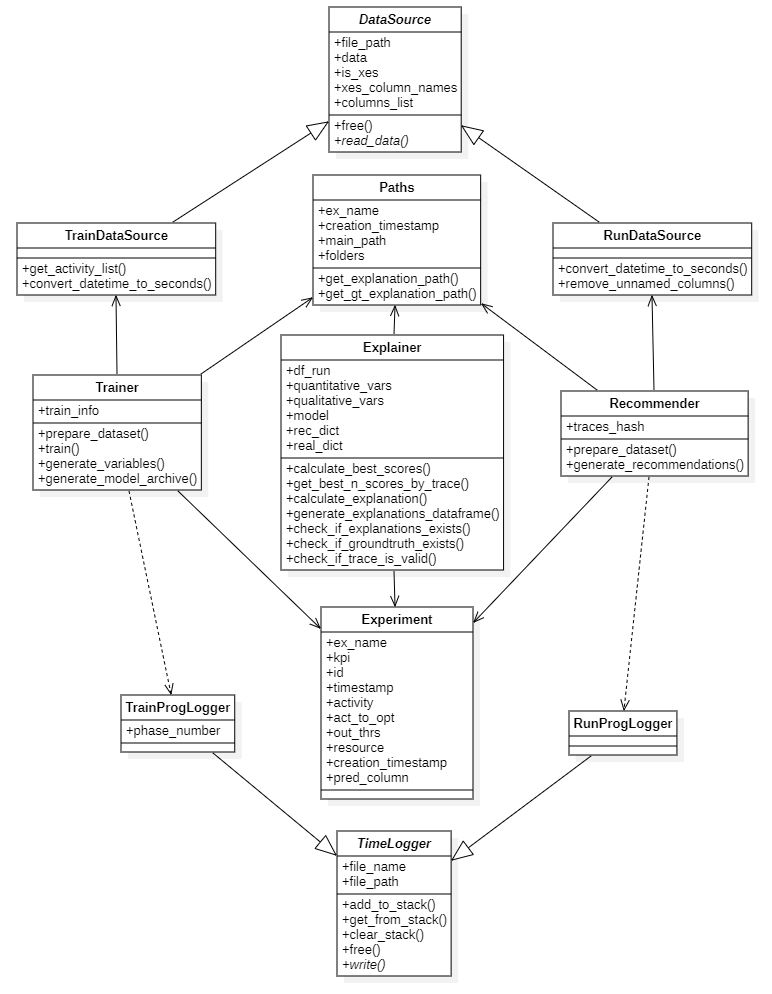
\includegraphics[width=1\columnwidth]{immagini/uml-model.jpg} 
    \caption{Diagramma UML per la classi del Model}
    \label{fig:uml-model}
\end{figure}



Del diagramma di classi in \autoref{fig:uml-model} si possono individuare le 3 classi principali, le cui responsabilità sono correlate alle 3 fasi descritte nella \autoref{sec:design-gui}:

\begin{itemize}
\item La classe \texttt{Trainer} che gestisce il processo di training e la memorizzazione dei dati generati su disco, in particolare sfrutta il metodo \texttt{prepare\_dataset} che si occupa di processare l'event log caricato per prepararlo al processo di training ed il metodo \texttt{train} che esegue il processo di training stesso per generare il process model;


\item La classe \texttt{Recommender} che gestisce il processo di generazione e memorizzazione delle raccomandazioni generate su disco. Anche per questa classe è necessario il metodo \texttt{prepare\_dataset} per processare l'event log caricato dall'utente e renderlo utilizzabile per il processo di generazione delle raccomandazioni che, a sua volta, viene eseguito dal metodo \texttt{generate\_recommendations};

\item La classe \texttt{Explainer} che si occupa della generazione, gestione e memorizzazione su disco delle spiegazioni per le raccomandazioni. Per far questo utilizza i dati prodotti dalle classi sopra descritte (ad esempio l'attributo \texttt{model} che rappresenta il process model generato) ed il metodo \texttt{calculate\_explanations} che genera le spiegazioni per una singola raccomandazione. Inoltre si occupa della visualizzazione delle raccomandazioni, generando le struttura dati che userà poi il componente View, usando i metodi \texttt{calculate\_best\_scores} e \texttt{get\_best\_n\_scores};

\end{itemize}

Le classi principali sopra descritte sfruttano a loro volta delle classi accessorie che si occupano di quelle funzionalità che, pur rimanendo necessarie, possono essere separate da quello che è il compito della classe principale. Esse sono:

\begin{itemize}
\item La classe \texttt{TrainDataSource} che viene usata dalla classe \texttt{Trainer} per la gestione dell'event log, infatti rappresenta la sorgente dei dati per il processo di training. Deriva dalla classe astratta \texttt{DataSource} di cui implementa il metodo \texttt{read\_data} che si occupa di leggere il file dell'event log dalla memoria. Alcuni attributi di nota sono, ad esempio, \texttt{data} che contiene i dati dell'event log in forma grezza e \texttt{columns\_list} che contiene tutti i nomi delle colonne presenti nell'event log. Offre i metodi \texttt{get\_activity\_list} per ottenere la lista di attività presenti nell'event log (necessita di sapere a quale colonna corrisponde la feature "activity") ed il metodo \texttt{convert\_datetime\_to\_seconds} per convertire i dati temporali della colonna relativa alla feature "timestamp" in secondi;

\item La classe \texttt{RunDataSource} che rappresenta la sorgente di dati relativi all'event log, per la classe \texttt{Recommender}. Essa ha la sua implementazione del metodo \texttt{read\_data} per la lettura del file dell'event log in memoria. Gli scopi sono paralleli a quelli della classe \texttt{TrainDataSource} e gli attributi hanno funzioni simili. Una differenza è la presenza del metodo \texttt{remove\_unnamed\_columns} che ripulisce l'event log di eventuali colonne vuote o senza identificativo che possono essere generate dopo aver letto i dati con il metodo \texttt{read\_data};

\item La classe \texttt{Experiment} è una classe senza metodi che contiene tutti i dati relativi all'esperimento corrente, ed esempio \texttt{ex\_name} identifica il nome dell'esperimento, \texttt{creation\_timestamp} il timestamp della creazione dell'esperimento mentre \texttt{id}, \texttt{timestamp}, \texttt{activity} e \texttt{resource} rappresentano colonne relative alle varie features richieste per gli event log. La classe viene usata da tutte e 3 le classi principali;

\item La classe \texttt{Paths} viene utilizzata da tutte e 3 le classi principali per la gestione di ogni percorso nel file system del server per i vari file usati per la memorizzazione dei dati generati, così da avere una sorgente univoca e facilitarne l'accesso e la modifica;

\item La classe \texttt{TrainProgLogger} che si occupa di gestire la visualizzazione del progresso del processo di training. Viene utilizzata dal metodo \texttt{train} della classe \texttt{Trainer};

\item La classe \texttt{RunProgLogger} che si occupa di gestire la visualizzazione del progresso del processo di generazione delle raccomandazioni. Viene utilizzata dal metodo \texttt{generate\_recommendations} della classe \texttt{Recommender}.

\end{itemize}


\subsection{Progettazione Presenter}
\label{subsec:presenter}
Per la progettazione del componente Presenter è stato tenuto conto della relazione tra singole view e singolo presenter, è stata definita una struttura a presenter multipli, che va a riflettere la struttura della componente View (\autoref{subsec:prog-views}).


\begin{figure}[H] 
    \centering 
    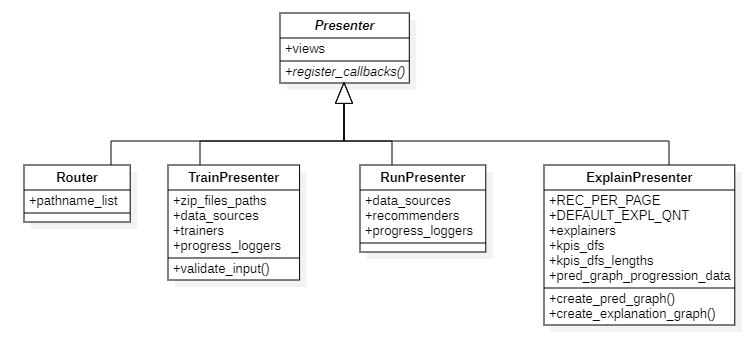
\includegraphics[width=0.8\columnwidth]{immagini/uml-presenters.jpg} 
    \caption{Diagramma UML per la classi del Presenter}
    \label{fig:uml-presenters}
\end{figure}

Lo scopo fondamentale del componente Presenter è la definizione delle callback per il framework Dash.
\\
Le callback rappresentano lo strumento offerto da Dash per sviluppare la componente interattiva di un'interfaccia grafica. 
\\
In una applicazione Dash gli input e output non sono altro che le proprietà dei vari componenti che formano il layout.
Le callback, sono delle funzioni Python che accettano una o più proprietà di specifici componenti come input e ritornano una o più proprietà di specifici componenti come output. Quando almeno una delle proprietà tracciate negli input viene modificata, la callback si avvia, esegue la sua logica interna e ritorna le modifiche alle proprietà di output, che vengono applicate al layout. 
\\ \\
Un esempio di callback:

\begin{lstlisting}[language=Python]
	@app.callback(
    Output(component_id='textout', component_property='value'),
    Input(component_id='textin', component_property='value')
)
def update_output(input_value):
    return input_value
\end{lstlisting}

In questo caso la callback \texttt{update\_output} verrà eseguita quando la proprietà \texttt{value} del componente con id \texttt{textin} verrà modificata. Al termine dell'esecuzione il valore in input verrà semplicemente ritornato e Dash si occuperà di aggiornare la proprietà \texttt{value} del componente con id \texttt{textout} con il nuovo testo.
\\ \\
Anche per progettazione del Presenter è stata sfruttata una classe astratta, la classe \texttt{Presenter}, che espone le funzionalità comuni per un singolo presenter, ovvero: 

\begin{itemize}

\item L'attributo \texttt{views} che contiene i vari riferimenti all'insieme delle view che il presenter può gestire;

\item Il metodo \texttt{register\_callbacks}, un metodo astratto che ogni istanza della classe \texttt{Presenter} deve implementare. Esso definisce tutte le callback che codificano il comportamento dell'interfaccia in risposta all'input dell'utente. 

\end{itemize}


Sono state definite 4 classi concrete che implementano la classe \texttt{Presenter}:

\begin{itemize}
\item La classe \texttt{Router} che gestisce principalmente la classe \texttt{BaseView} della componente View, quindi si occupa di tutti gli aspetti relativi al cambio di pagina. L'attributo \texttt{pathname\_list} è definito in automatico e contiene gli identificativi di tutte le altre view, ordinate secondo il loro attributo \texttt{order}.

\item La classe \texttt{TrainPresenter} che gestisce la classe \texttt{TrainView} della componente View. Si interfaccia con il componente Model per l'esecuzione del processo di training. Per fare questo vengono utilizzati gli attributi \texttt{trainers}, \texttt{data\_sources} e \texttt{progress\_loggers} che rappresentano le istanze delle classi \texttt{Trainer}, \texttt{TrainDataSource} e \texttt{TrainProgLogger} della componente Model. Poiché la pagina della fase di training accetta l'input dell'utente è stato definito il metodo \texttt{validate\_input} che ne gestisce la validazione;

\item La classe \texttt{RunPresenter} che gestisce la classe \texttt{RunView} della componente View. Anche questa classe necessita di interfacciarsi con il componente Model per gestire l'esecuzione del processo di generazione delle raccomandazioni. Sfrutta gli attributi \texttt{recommenders}, \texttt{data\_sources} e \texttt{progress\_loggers} che rappresentano le istanze delle classi \texttt{Recommender}, \texttt{RunDataSource} e \texttt{RunProgLogger} della componente Model.

\item La classe \texttt{ExplainPresenter} che gestisce la classe \texttt{RunView} della componente View. Quindi gestisce la generazione delle spiegazioni, tramite la componente Model, sfruttando, in particolare l'attributo \texttt{explainers} che rappresenta le istanze della classe \texttt{Explainer}. Si occupa anche della visualizzazione delle raccomandazioni e delle spiegazioni, sfruttando il metodo \texttt{create\_pred\_graph} per generare il grafico delle raccomandazioni ed il metodo \texttt{create\_explanation\_graph} per generare il grafico delle spiegazioni. Il resto degli attributi è usato per gestire la visualizzazione dei grafici.

\end{itemize}

\subsection{Struttura cartelle per il salvataggio dei file su disco}
Come da requisiti, era necessario il salvataggio di tutti i dati relativi al process model generato, alle raccomandazioni e alle spiegazioni, per ogni esperimento eseguito. La scelta più semplice era appunto salvarli su disco, ovvero sulla memoria permanente del server.
\\
Di seguito l'organizzazione delle cartelle che è stata progettata:
\\ \\
\begin{forest}
  for tree={
    font=\ttfamily,
    grow'=0,
    child anchor=west,
    parent anchor=south,
    anchor=west,
    calign=first,
    edge path={
      \noexpand\path [draw, \forestoption{edge}]
      (!u.south west) +(7.5pt,0) |- node[fill,inner sep=1.25pt] {} (.child anchor)\forestoption{edge label};
    },
    before typesetting nodes={
      if n=1
        {insert before={[,phantom]}}
        {}
    },
    fit=band,
    before computing xy={l=15pt},
  }
[experiments
  [test\_experiment1
    [archives]
    [explanations]
    [model]
    [recommendations]
    [results]
    [variables]
    [experiment\_info.json]
  ]
]
\end{forest}

La struttura sopra rappresenta un ipotetico esperimento nominato "test\_experiment1". 
In particolare sono definiti i seguenti elementi:

\begin{itemize}
\item \texttt{archives} è una cartella che contiene l'archivio compresso di tutti i dati del process model. Questo può venir scaricato dall'utente al termine del processo di training, se lo desidera;

\item \texttt{explanations} è una cartella che contiene tutte le spiegazioni generate;

\item \texttt{model} è una cartella che contiene tutti i dati relativi al process model;

\item \texttt{recommendations} è una cartella che contiene tutti i dati relativi alle raccomandazioni generate;

\item \texttt{results} è una cartella che contiene alcune delle metriche calcolate durante il processo di training;

\item \texttt{variables} è una cartella che contiene i dati relativi alle variabili qualitative e quantitative generate al termine del processo di training;

\item \texttt{experiment\_info.json} è un file che contiene tutti i dati relativi all'esperimento (nome, timestamp di creazione, KPI scelto e features).

\end{itemize}


\section{Codifica}

\subsection{Sviluppo della modalità wizard}

Prima di tutto è stata sviluppato il sistema per attuare la modalità wizard, che definisce l'aspetto base dell'interfaccia: una procedura a fasi ordinate, dove ad ogni singola fase corrisponde una pagina, con la possibilità di navigare tra le pagine tramite un comando che permette di andare alla pagina successiva ed un comando che permette di andare alla pagina precedente. Questo meccanismo rappresenta lo scheletro dell'interfaccia.

\begin{figure}[H] 
    \centering 
    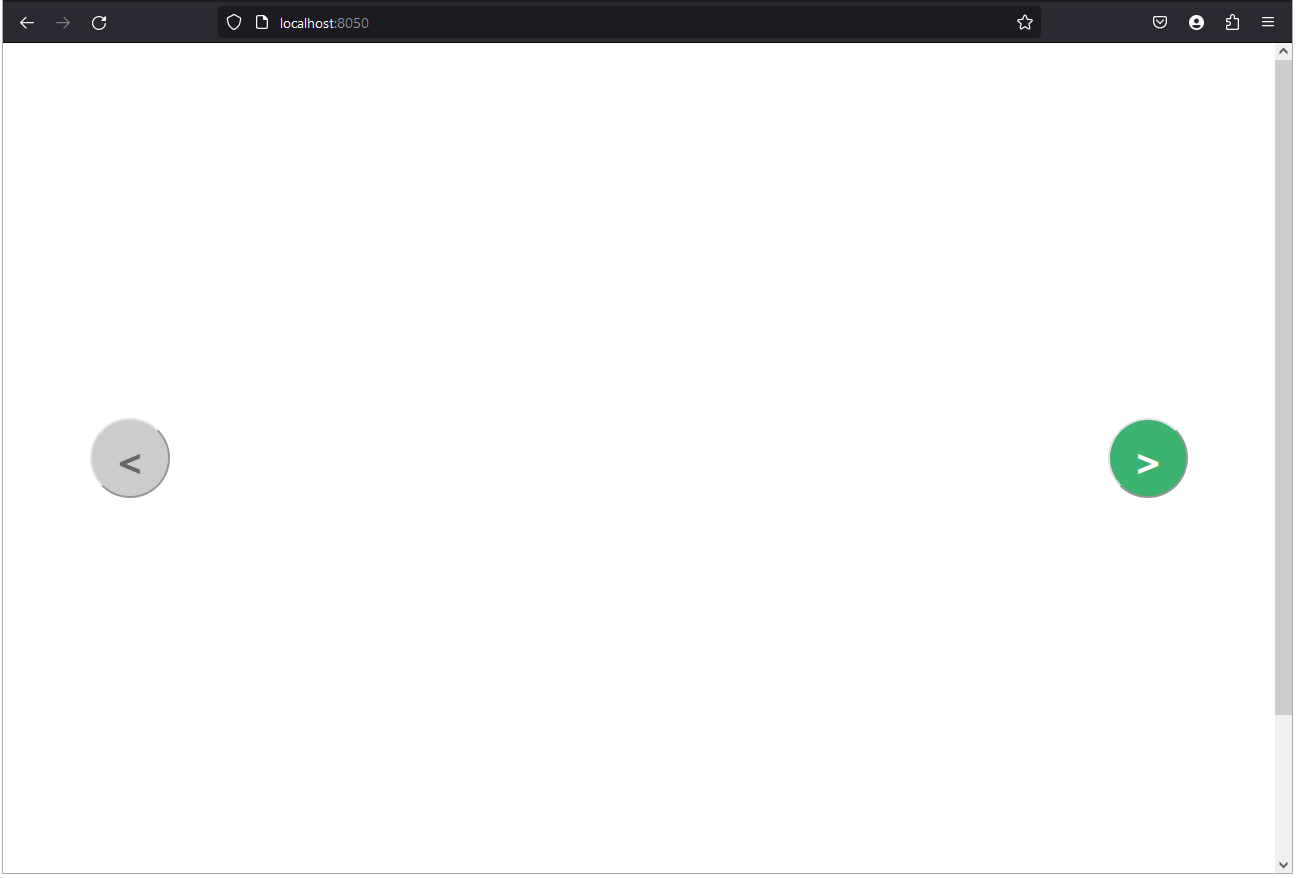
\includegraphics[width=0.8\columnwidth]{immagini/pag-baseview.png} 
    \caption{Comandi wizard}
    \label{fig:pag-baseview}
\end{figure}

L'aspetto del sistema viene raffigurato in \autoref{fig:pag-baseview}, in particolare si possono notare i due bottoni per navigare le pagine come descritto sopra.
\\
Il funzionamento è semplice: viene monitorato l'url, e ad ogni sua modifica, una callback estrae il percorso e verifica se esso combacia con l'attributo \texttt{pathname} di una delle view, in caso positivo il layout della view viene mostrato in un elemento contenitore. I pulsanti di navigazione servono a modificano l'url con il percorso corretto.
Infine il sistema supporta la funzionalità di disabilitazione dei comandi di navigazione, per esempio se ci sono delle condizioni da superare per andare alla pagina successiva. Tutto ciò è gestito dal presenter \texttt{Router}.

Il layout invece è definito nella view \texttt{BaseView}. Esso è stata partizionato in 3 sezioni: due laterali per i comandi di navigazione e una sezione centrale che ospita l'elemento contenitore di cui si è parlato in precedenza.


\subsection{Sviluppo della pagina per la fase di training}
Per lo sviluppo della pagina per la fase di training sono state apportate alcune modifiche grafiche e funzionali alla versione progettata inizialmente.

\subsubsection{Componente per il caricamento degli event log}
\phantomsection
\label{subsubsec:dash-uploader}

\begin{figure}[H] 
    \centering 
    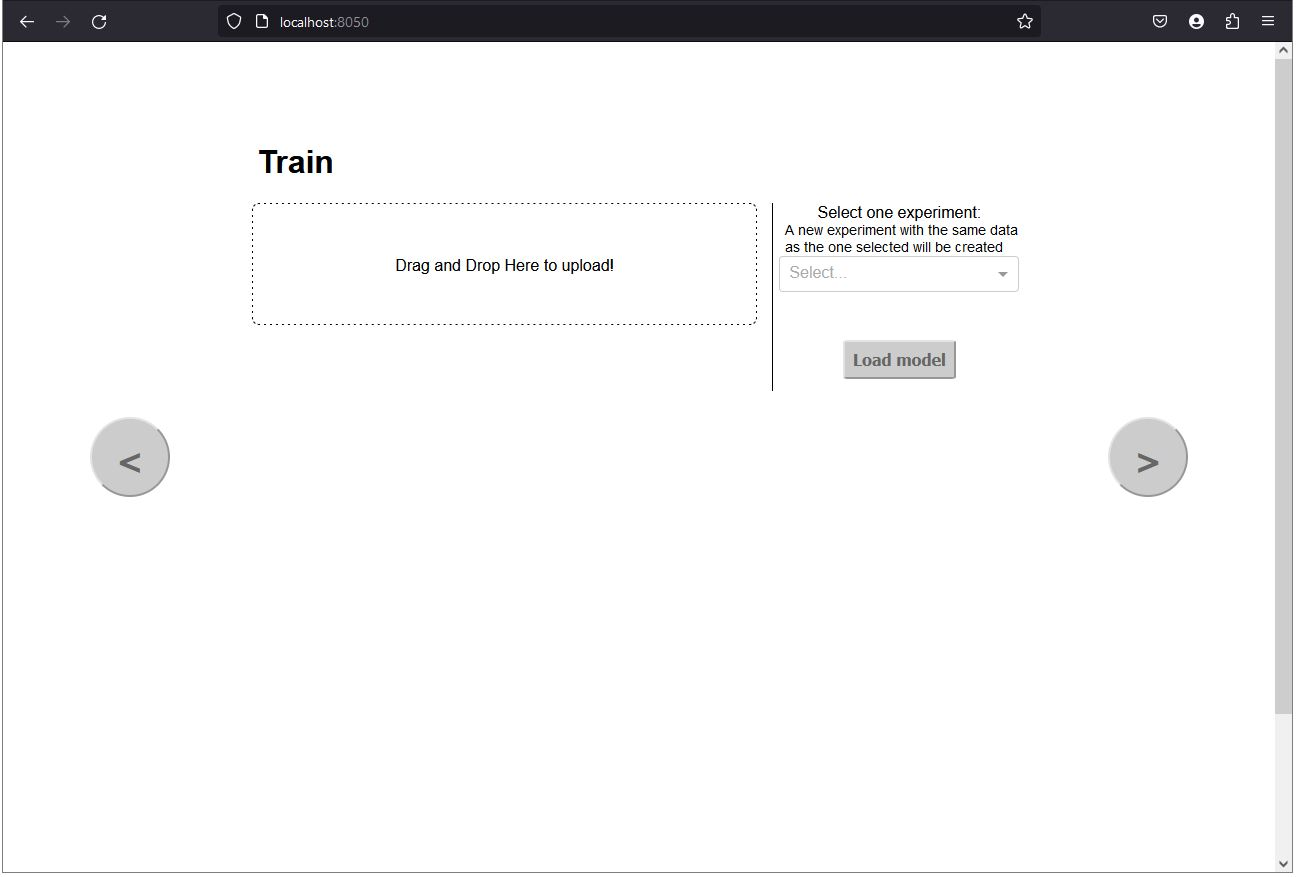
\includegraphics[width=0.7\columnwidth]{immagini/train-pag-no-event-log.jpg} 
    \caption{Pagina fase di training senza nessun event log caricato}
\end{figure}

Un'importante modifica riguarda il componente \gls{drag-and-drop} per caricare gli event log. Inizialmente si era pensato di utilizzare il componente \texttt{Upload} offerto da Dash nei suoi componenti base. Ma questo componente aveva una grossa restrizione: pur essendo in teoria capace di gestire file di dimensioni arbitrariamente grandi, nella pratica la dimensione massima dei file gestibili era limitata a circa 150MB mentre la dimensione consigliata era intorno ai 10MB \cite{site:upload-max-size}. 
\\
Questo è dovuto al funzionamento del componente che prima converte il file in una stringa \gls{base64} caricandolo nella memoria locale del browser e, successivamente, carica la stringa generata nella memoria permanente del server. Se il file da caricare è troppo grande la saturazione della memoria locale porta in browser a stalli e/o terminazioni improvvise.
\\
Si è quindi deciso di utilizzare il componente \texttt{dash-uploader} \cite{site:dash-uploader}, sviluppato e mantenuto dalla community. Esso infatti risolve la restrizione riscontrata poiché esegue il caricamento del file a blocchi di dimensioni ridotte direttamente sulla memoria permanente del server. L'unica limitazione di dimensioni diventa quindi la dimensione del disco rigido del server.

\subsubsection{Inserimento delle opzioni di training}

\begin{figure}[H] 
    \centering 
    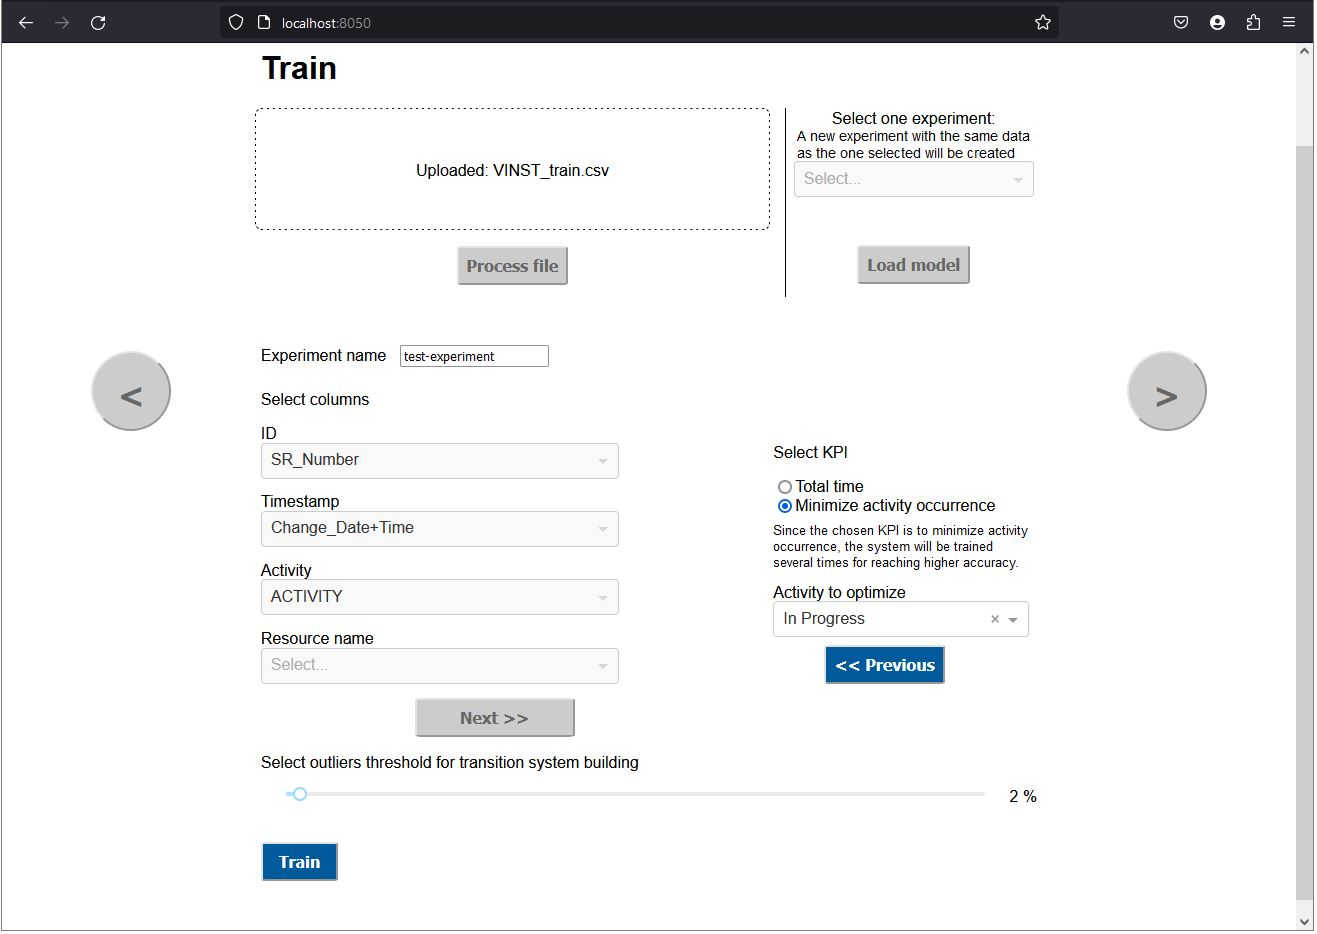
\includegraphics[width=0.7\columnwidth]{immagini/pag-train-loaded-event-log.jpg} 
    \caption{Pagina fase di training con un event log caricato e tutte le opzioni di training inserite}
    \label{fig:opzioni-training}
\end{figure}

\begin{figure}[H] 
    \centering 
    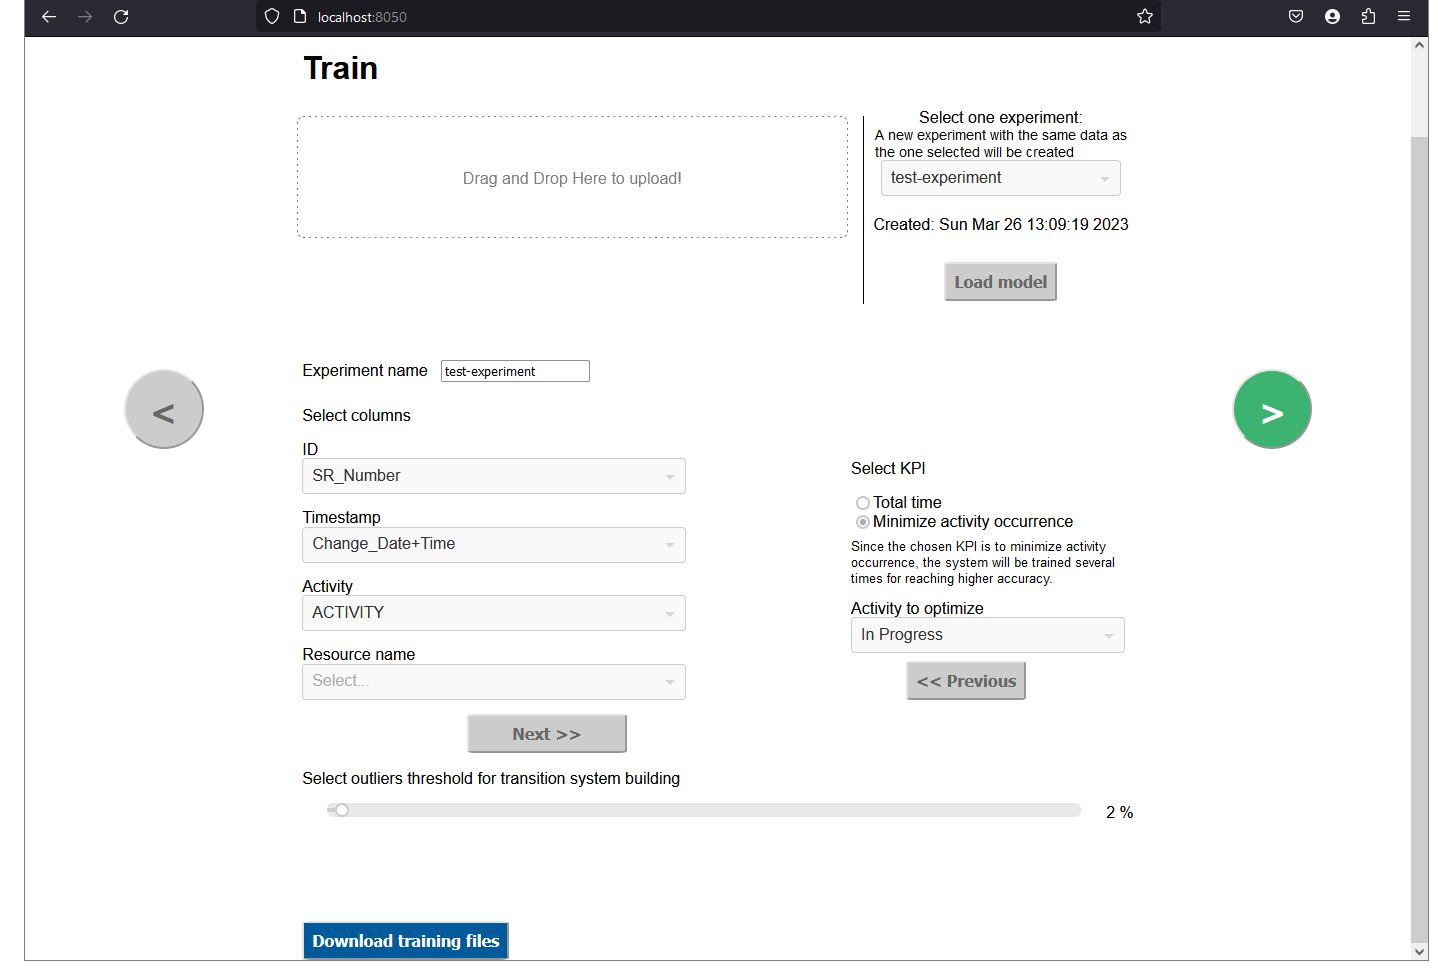
\includegraphics[width=0.7\columnwidth]{immagini/pag-train-model-loaded.jpg} 
    \caption{Pagina fase di training con caricato un process model già allenato}
    \label{fig:caricamento-modello}
\end{figure}

L'interfaccia responsabile per l'inserimento delle opzioni di training ha subito alcuni cambiamenti. Vista la necessità di seguire il flusso di esecuzione descritto nella \autoref{subsec:training-phase} (in particolare i passi 2 e 3 del flusso principale), sono stati inseriti dei bottoni aggiuntivi che permettono di cambiare "fase" di compilazione solo dopo aver completato quella corrente.
Fintanto che una fase non è accessibile tutti i componenti che la costituiscono rimangono disabilitati, come si può notare in \autoref{fig:opzioni-training}.\\
Questo si è reso necessario per facilitare la compilazione, per ridurne gli errori e per permettere all'interfaccia di conoscere la colonna corrispondente alla feature "activity" così da poter elencare le attività corrette nel \gls{dropdown} "Activity to optimize" nel caso in cui si sia scelto il KPI "Minimize activity occurrence".
\\
Un altro cambiamento da considerare riguarda quei casi di utilizzo in cui i controlli vengono usati per la sola visualizzazione delle opzioni.
Questo accade quando l'utente usa un event log in formato XES, dove le feature sono già definite implicitamente nella codifica del file, e quando l'utente carica un process model già allenato (come nel caso in \autoref{fig:caricamento-modello}), per il quale tutte le opzioni sono già state specificate in un momento precedente. In questi casi, i controlli le cui le opzioni sono già determinate rimangono \textit{read-only}, cioè non modificabili. 


\subsubsection{Visualizzazione del progresso del processo di training}
\phantomsection
\label{subsubsec:progress-train}

\begin{figure}[H] 
    \centering 
    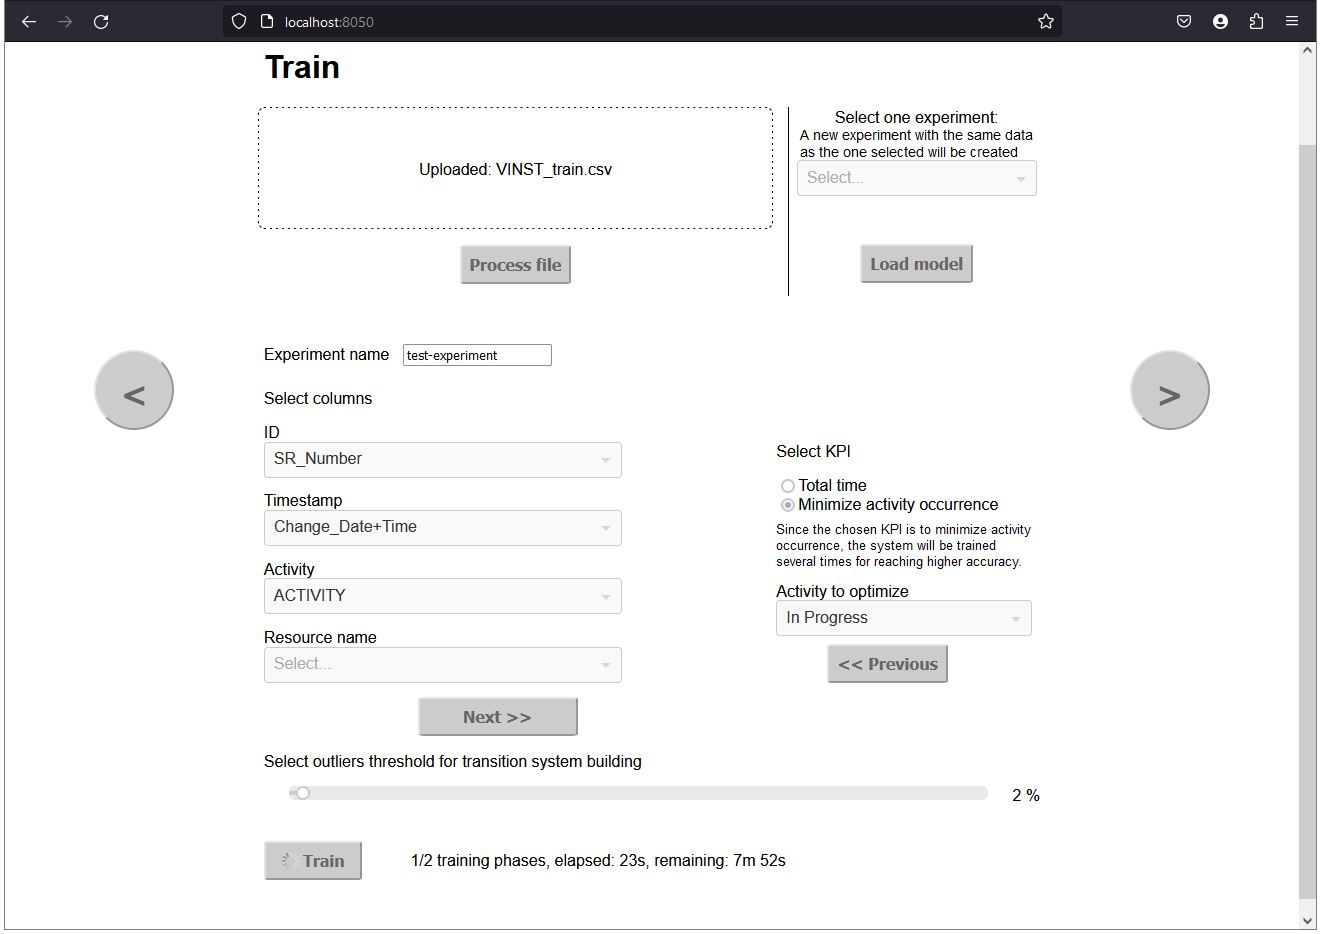
\includegraphics[width=0.7\columnwidth]{immagini/pag-train-started-training.jpg} 
    \caption{Pagina fase di training con il processo di training avviato}
    \label{fig:progresso-train}
\end{figure}

Innanzitutto va precisato che il processo di training è suddiviso in 3 fasi:

\begin{itemize}
\item Preparazione dell'event log per la fase di training;

\item Processo di training effettivo;

\item Generazione di variabili qualitative e quantitative.

\end{itemize}
L'interesse principale viene posto nella seconda fase, che è quella che richiede più tempo. Per questo, il tempo impiegato dalla prima e dalla terza fase può essere trascurato.
\\
La seconda fase, il training effettivo, è basato sulla funzione \texttt{fit} di della libreria Catboost \cite{site:catboost-fit}. L'unica possibilità per avere una corretta indicazione del progresso del processo di training era l'utilizzo del parametro \texttt{logging\_level="Verbose"} offerto dalla funzione. 
\\
Il parametro stampa nell'output standard varie informazioni relative al training. Quelle utilizzate per tracciare il progresso del training sono: l'indicazione di quanto tempo è passato dall'avvio delle funzione e l'indicazione, stimata, del tempo rimanente al termine della funzione.
\\
L'idea iniziale per la visualizzazione del progresso del processo di training era l'utilizzo di una barra di caricamento.
Però è chiaro come queste informazioni temporali, stimate, avrebbero reso un'eventuale barra di caricamento molto instabile, dato che fluttuazioni dei tempi indicati avrebbero portato ad improvvisi spostamenti in avanti o indietro della barra stessa. Si è quindi optato per un'indicazione testuale delle informazioni temporali che si aggiorna ad intervalli regolari (come si pò vedere in \autoref{fig:progresso-train}).
\\
Per poter utilizzare queste informazioni era necessario reindirizzare l'output su un file temporaneo.  Per fare questo la funzione \texttt{fit} offriva già un altro parametro apposito, \texttt{log\_cout}. Specificando il nome del file temporaneo la funzione avrebbe stampato le informazioni al suo interno e questo avrebbe permesso all'interfaccia di accedervi in maniera più comoda.
\\
L'accesso al suddetto file è mediato dalla classe \texttt{TrainProgLogger}: ad intervalli regolari il sistema preleva l'informazione grezza più recente dal file (interfacciandosi con \texttt{TrainProgLogger}), questa poi viene analizzata e ripulita e infine viene mostrata nell'interfaccia grafica.


%\hyperref[subsubsec:progress-train]{Test}

\subsection{Sviluppo della pagina per la fase di runtime}
Lo sviluppo della pagina di runtime non ha richiesto particolari modifiche di carattere grafico alla versione progettata inizialmente.
\\ 
Ad ogni modo, visto che la pagina necessitava del caricamento di un'event log tramite un componente \gls{drag-and-drop}, è stato usato di nuovo il componente \texttt{dash-uploader}, facendo le stesse considerazioni fatte in precedenza (vedi paragrafo \hyperref[subsubsec:dash-uploader]{Componente per il caricamento degli event log}).


\begin{figure}[H] 
    \centering 
    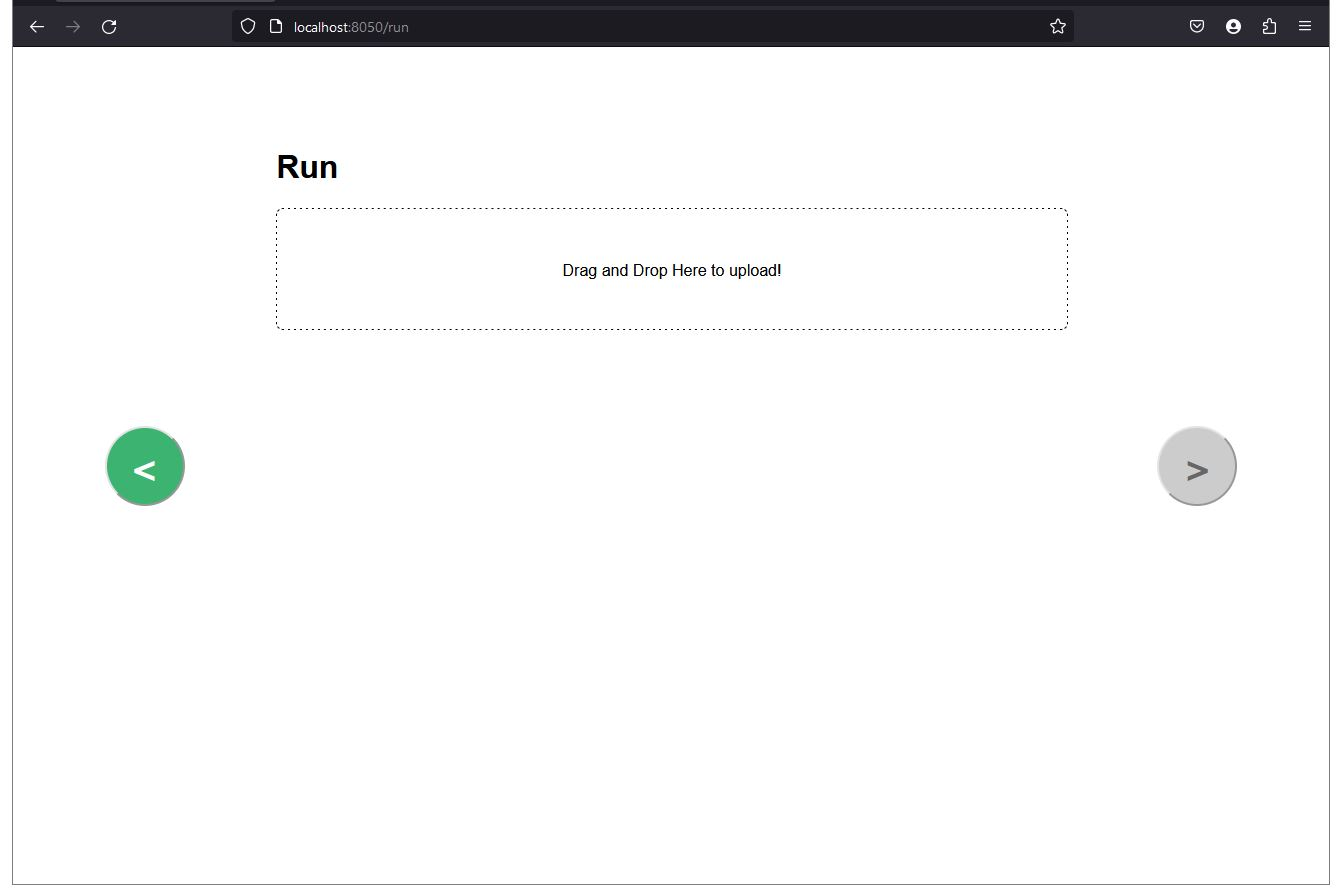
\includegraphics[width=0.7\columnwidth]{immagini/pag-run-no-event-log.jpg} 
    \caption{Pagina fase di runtime senza nessun event log caricato}
\end{figure}

\begin{figure}[H] 
    \centering 
    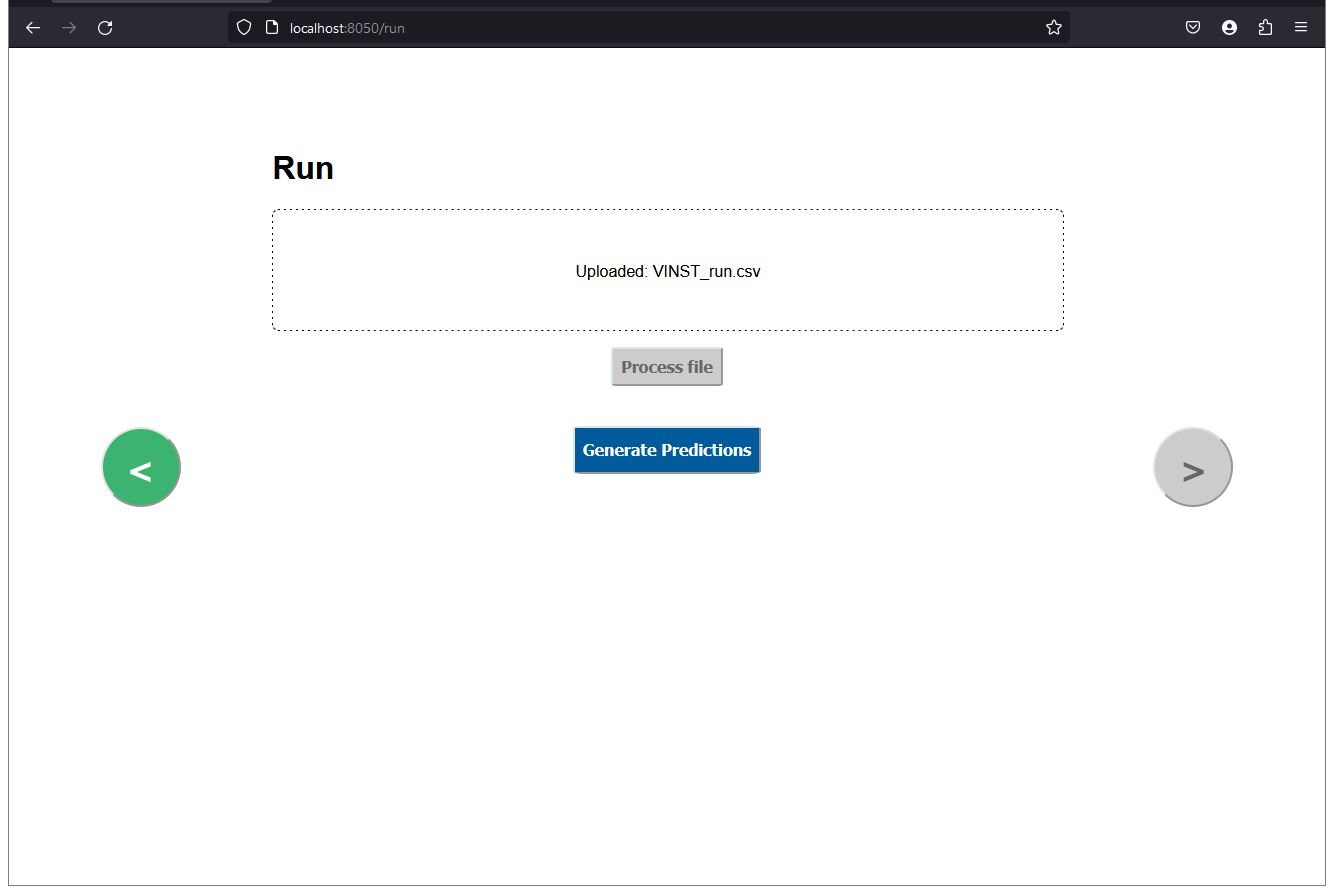
\includegraphics[width=0.7\columnwidth]{immagini/pag-run-loaded-event-log.jpg} 
    \caption{Pagina fase di runtime con un event log caricato}
\end{figure}

\subsubsection{Visualizzazione del progresso del processo di generazione delle raccomandazioni}

\begin{figure}[H] 
    \centering 
    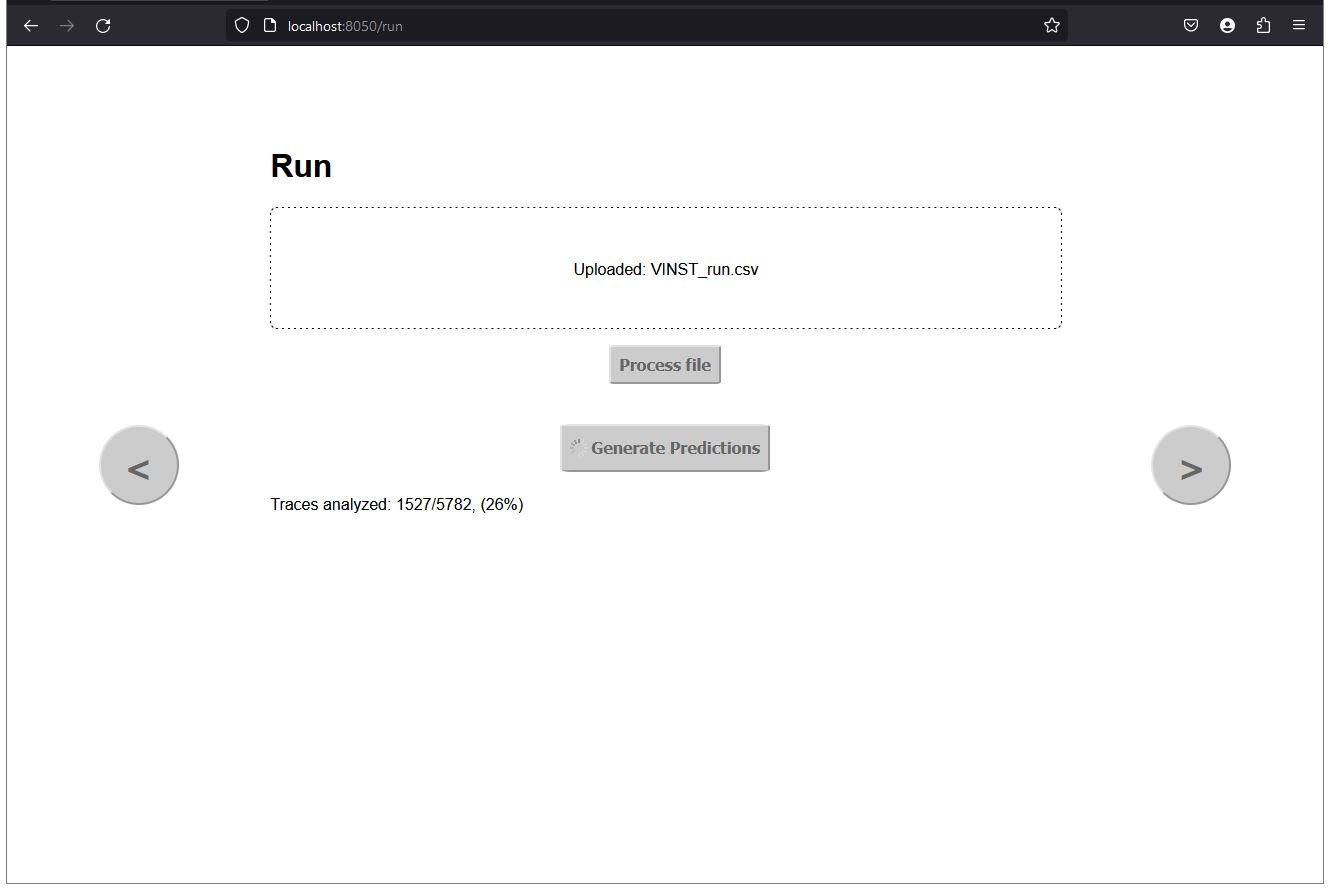
\includegraphics[width=0.7\columnwidth]{immagini/pag-run-recommendation-generation.jpg} 
    \caption{Pagina fase di runtime con il processo di generazione delle raccomandazioni avviato}
    \label{fig:progresso-run}
\end{figure}

In questo caso il processo di generazione delle raccomandazioni itera sulle tracce dell'event log caricato ed è implementato direttamente nel back-end del sistema, quindi una barra di progresso era di facile implementazione.
\\
Però, per evitare di cambiare modalità di visualizzazione rispetto alla pagina precedente, si è deciso di utilizzare ancora l'indicazione testuale del progresso. 
\\
Per far questo è stato utilizzato un principio simile a quanto descritto nel paragrafo \hyperref[subsubsec:progress-train]{Visualizzazione del progresso del processo di training}. Viene sfruttato l'output della libreria \texttt{tqdm} \cite{site:tqdm} applicata all'iterazione principale, che è poi reindirizzato su un file temporaneo. Quest'ultimo viene letto ad intervalli periodici acquisendo le informazioni grezze più recenti che vengono filtrate. Vengono estratti i dati relativi al progresso in percentuale, alle tracce analizzate e alle tracce totali. Infine le informazioni vengono riscritte in un formato più leggibile e mostrate nell'interfaccia grafica (come in \autoref{fig:progresso-run}). 
\\
La classe \texttt{RunProgLogger} si occupa dell'accesso al file temporaneo e della manipolazione dell'informazione grezza.


\subsection{Sviluppo della pagina per la fase di visualizzazione}
Anche per lo sviluppo della pagina di visualizzazione sono state necessarie alcune modifiche, sia grafiche che funzionali, rispetto a quanto progettato.

\subsubsection{Paginazione per il grafico di visualizzazione delle raccomandazioni}

\begin{figure}[H] 
    \centering 
    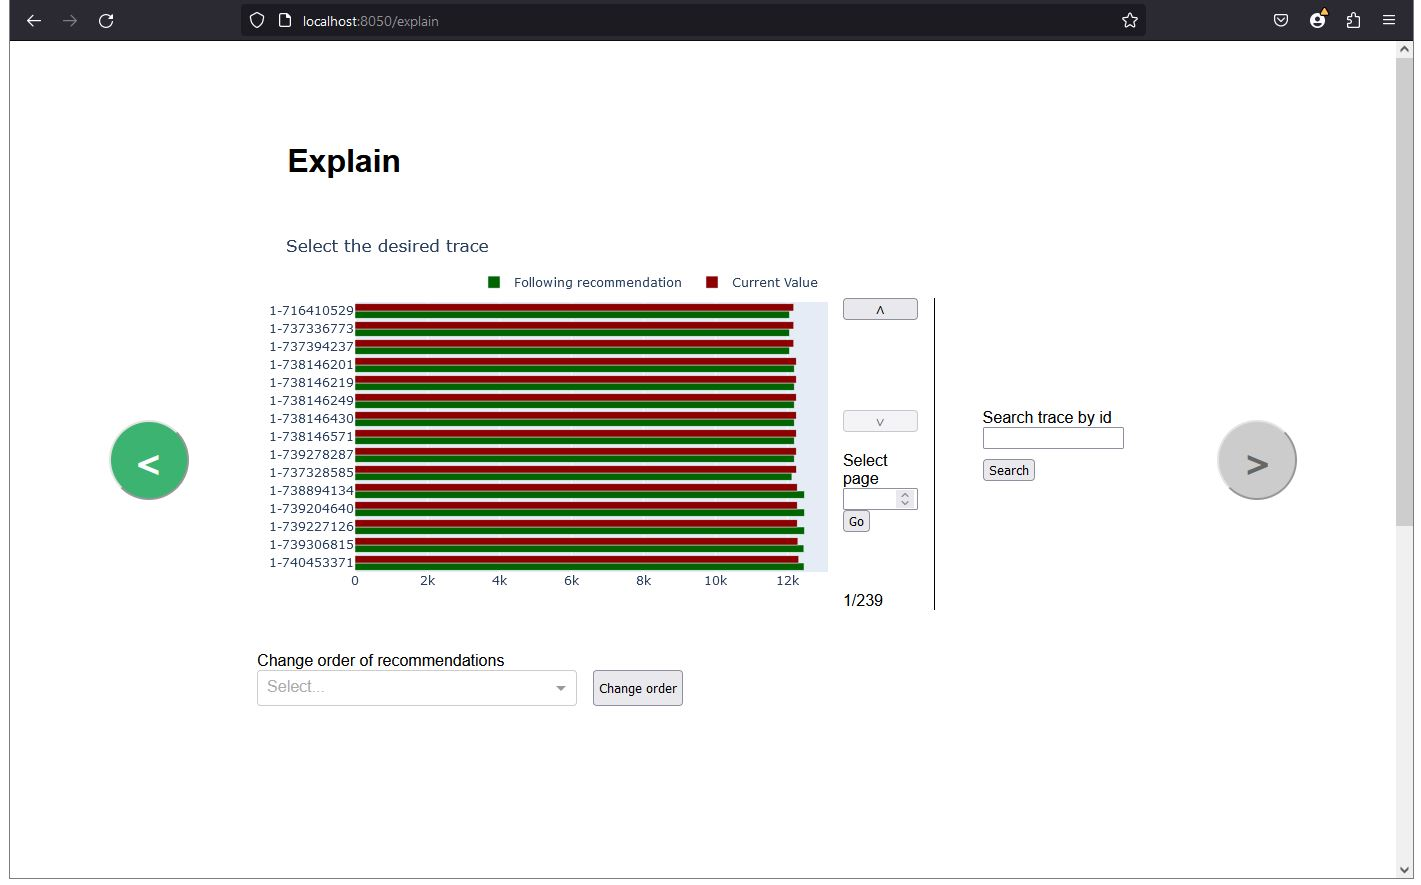
\includegraphics[width=0.7\columnwidth]{immagini/pag-explain-first-access.jpg} 
    \caption{Pagina fase di visualizzazione senza nessuna raccomandazione selezionata}
    \label{fig:explain-paginazione}
\end{figure}

Durante la progettazione non si è considerato il problema che riguardava la visualizzazione di molte raccomandazioni nel grafico. Infatti esso diventava illeggibile anche andando oltre le 20 raccomandazioni visualizzate. 
\\
Considerando quindi che il numero tipico di raccomandazioni sarebbe stato di gran lunga maggiore e che le dimensioni del grafico dovevano rimanere quelle decise in sede di progettazione, la soluzione pensata richiedeva la necessità di paginare il grafico.
\\
Il dataset contenente l'insieme delle raccomandazioni viene suddiviso in porzioni di dimensione fissata a 15 e queste porzioni, o pagine, vengono visualizzate nel grafico una alla volta. Per la navigazione delle pagine sono stati sviluppati alcuni comandi aggiuntivi (possono essere visualizzati nella \autoref{fig:explain-paginazione}):

\begin{itemize}
\item Un indicatore della pagina attuale e del numero totale di pagine;

\item Due pulsanti per passare alla pagine successiva o precedente;

\item Un pulsante per andare ad una specifica pagina dopo averne specificato il numero.

\end{itemize}

In questo modo è stata resa possibile la visualizzazione di un numero di raccomandazioni arbitrariamente grande.

\subsubsection{Miglioramento della visualizzazione testuale delle raccomandazioni}
\begin{figure}[H] 
    \centering 
    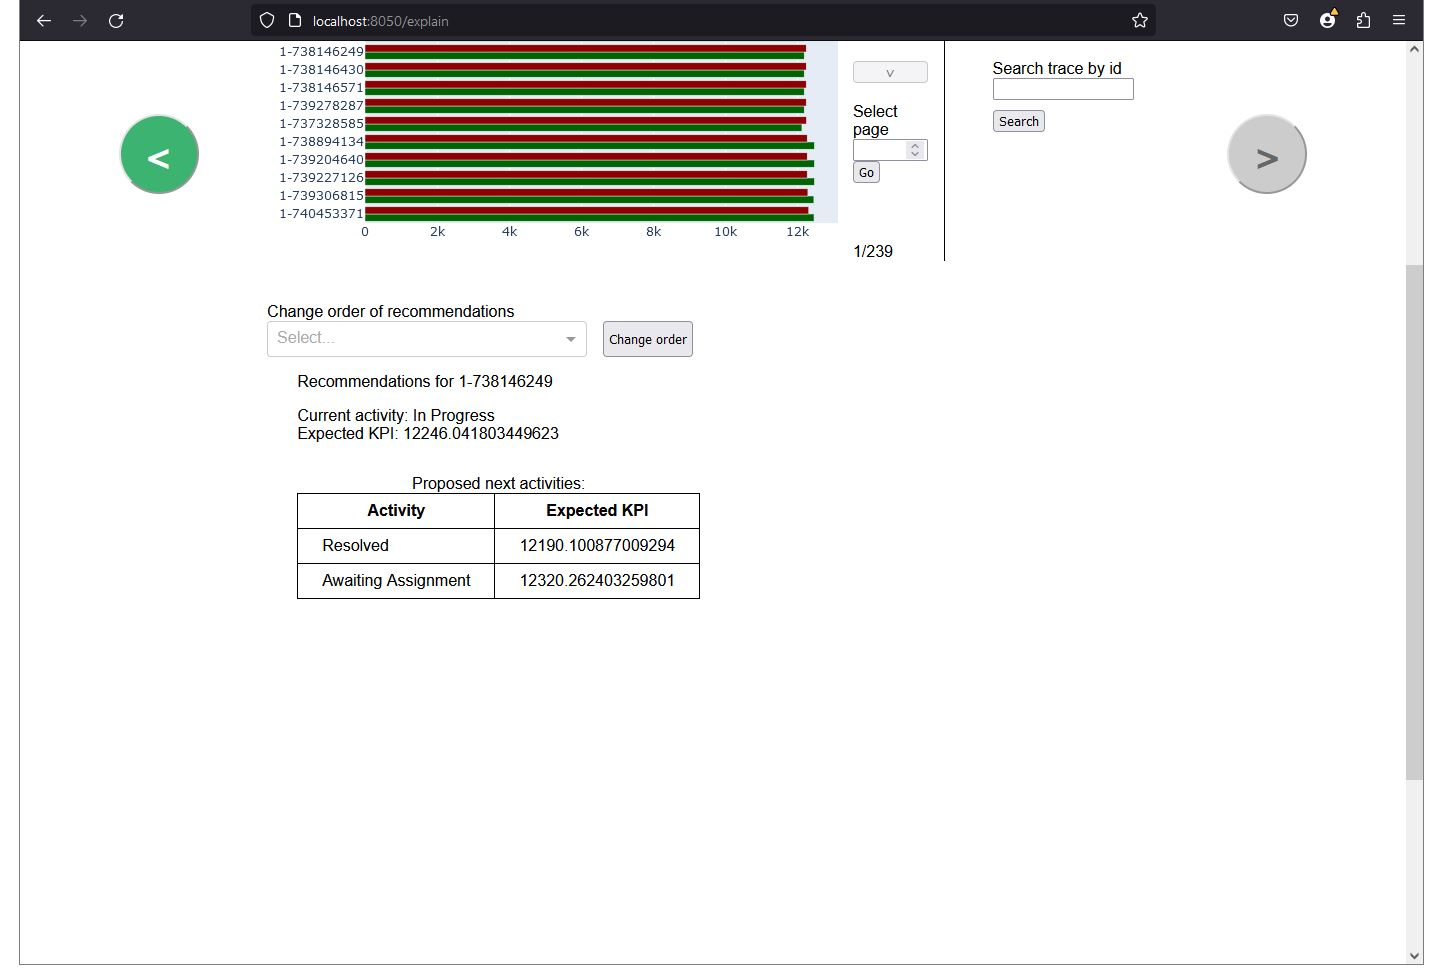
\includegraphics[width=0.7\columnwidth]{immagini/pag-explain-selected-trace.jpg} 
    \caption{Pagina fase di visualizzazione con raccomandazione selezionata}
\end{figure}

\begin{figure}[H] 
    \centering 
    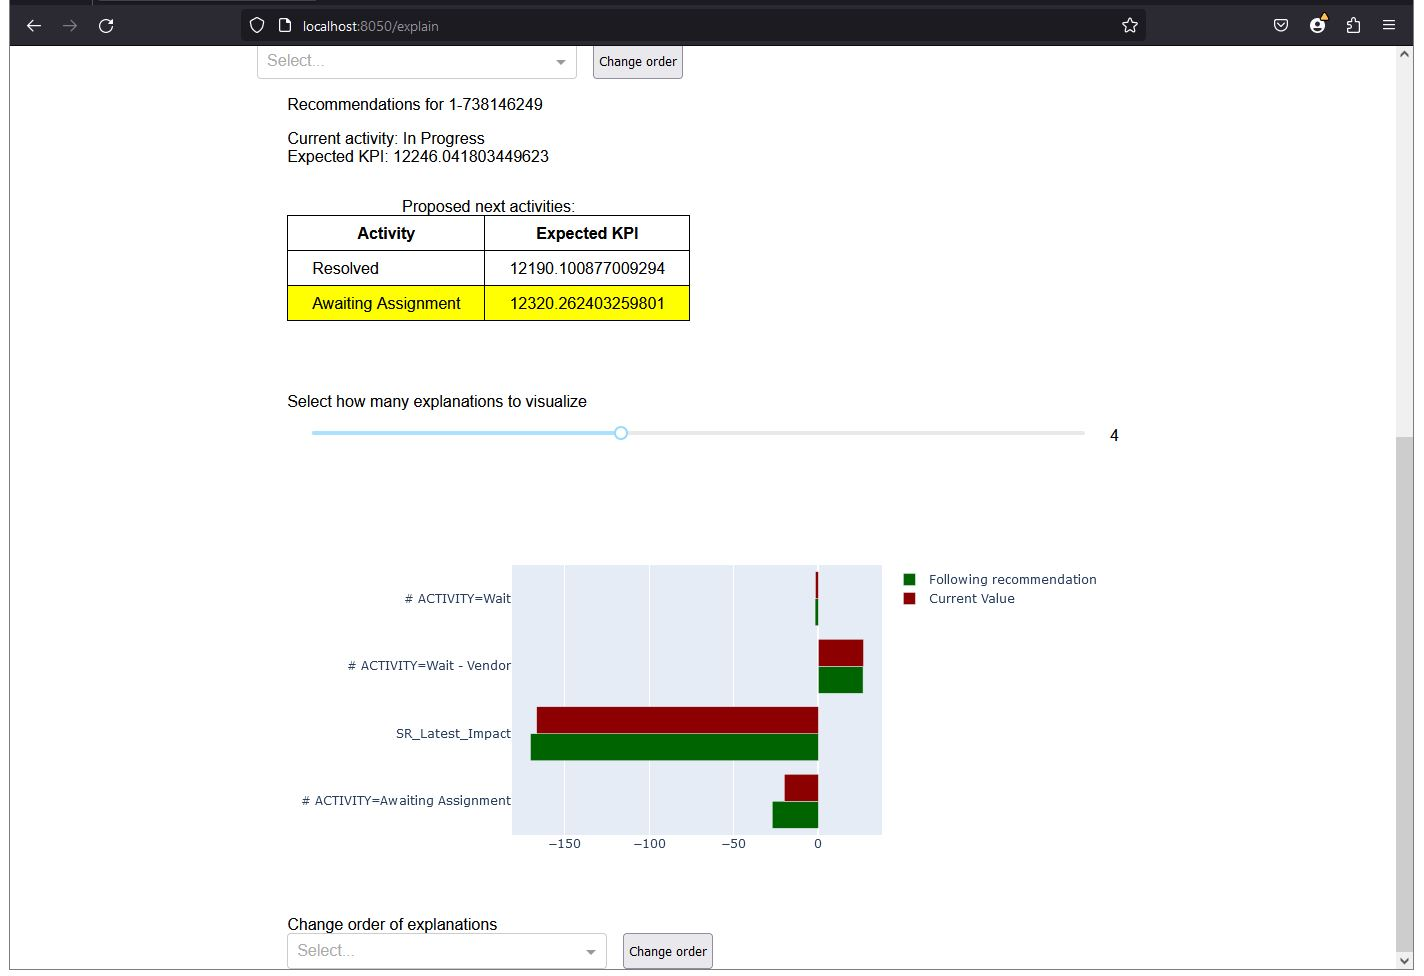
\includegraphics[width=0.7\columnwidth]{immagini/pag-explain-explanations.jpg} 
    \caption{Pagina fase di visualizzazione con spiegazione generate}
\end{figure}

Come visto nella progettazione il sistema genera un massimo di 3 raccomandazioni per traccia, la migliore viene mostrata nel grafico e il resto può essere visionato, in forma testuale, selezionando la traccia.
Si è deciso di aggiungere altri dati, per migliorare la comprensione da parte dell'utente. Essi sono:

\begin{itemize}
\item L'identificativo della traccia selezionata;

\item L'attività attuale, ovvero l'attività a cui è arrivata la traccia nell'event log caricato nella fase di runtime;

\item Il KPI medio predetto, inteso come il KPI che ci si aspetta al completamento della traccia senza considerare le raccomandazioni, quindi il KPI da migliorare.

\end{itemize}


\subsection{Utilizzo delle background callback di Dash}
Dash offre un'interessante funzionalità per le callback le cui computazioni mediamente superano i 10/20 secondi. Esse infatti possono causare errori improvvisi e comportamenti non definiti determinati dal periodo di timeout imposto alle richieste HTTP. Può succedere infatti che, alla scadenza del timeout, la callback fallisca silenziosamente l'esecuzione.
\\ 
Da notare come questo periodo di timeout dipenda dalla macchina su cui si esegue il back-end, quindi non c'è un modo sicuro e indipendente dalla piattaforma di gestire questo parametro. Inoltre è sconsigliato aumentarlo, poiché potrebbe portare ad un esaurimento delle risorse disponibili e mandare in stallo l'applicazione.
\\
Per rimediare a questo Dash offre il meccanismo delle background callback \cite{site:dash-background-callbacks}.
Il funzionamento è semplice: la richiesta di esecuzione della callback viene inserita in una coda. Quando arriva il suo turno, viene fatta eseguire su un processo secondario e periodimente viene inviata una richiesta per controllare se ha terminato. Questo permette di evitare il problema del timeout.
\\ \\
I processi computazionali, che possono richiedere una considerevole quantità di tempo, e che quindi necessitano di queste particolari callback sono:

\begin{itemize}
\item L'analisi e l'elaborazione al caricamento dell'event log per la fase di training;

\item Il processo di training;

\item L'analisi e l'elaborazione al caricamento dell'event log per la fase di runtime;

\item Il processo di generazione delle raccomandazioni;

\item Il processo di generazione delle spiegazioni.

\end{itemize}

Le background callback possono richiedere una breve attesa prima di poter essere eseguite, visto che esse sono poste in una coda. Ad esempio, che se l'utente preme un pulsante che avvia una background callback, ci possono volere alcuni secondi perché l'interfaccia risponda. Questo può causare confusione all'utente, spingendolo a premere multiple volte il pulsante.
\\ 
Per evitare questa situazione è stata aggiunta un'ulteriore funzionalità, per ognuno di questi bottoni che avviano una background callback: la disabilitazione del comando stesso e la comparsa di un "indicatore di attesa". Un esempio è il pulsante "Train" in \autoref{fig:progresso-run}.

\subsection{Sviluppo delle funzionalità multiutente}
L'idea iniziale per l'interfaccia era che essa fosse utilizzabile solo da un singolo utente, che avrebbe installato ed utilizzato il sistema in maniera autonoma. Per questa ragione il sistema è stato progettato e sviluppato interamente secondo una prospettiva a singolo utente. 
\\
Solo in un momento successivo, si è considerata la possibilità di estendere il sistema per renderlo multiutente, pur considerando l'aggiunta di questa nuova funzionalità desiderabile e non obbligatoria (vedi \autoref{sec:stage-obj}).
\\
L'obiettivo era quindi andare a trasformare un sistema a singolo utente, già funzionante, in multiutente, riducendo al minimo le modifiche al codice già scritto. Questo si è reso necessario per evitare di dover riprogettare e re-implementare il sistema per intero, dato che non era compatibile con i tempi prefissati di durata dello stage.


\subsubsection{Il problema principale}
Il framework Dash offre nativamente la capacità di supportare utenti multipli, ad una condizione: la componente server deve essere \textit{stateless}. Questo significa che l'applicazione non deve salvare dati generati dall'utente, dati di sessioni precedenti o dati di computazioni precedenti. 
\\
Come spiegato nella documentazione \cite{site:dash-stateless}, Dash scala in maniera orizzontale, quindi, per poter gestire più utenti, vengono eseguite più istanze della stessa applicazione in più processi paralleli. Da notare come non ci sia una associazione uno a uno tra una sessione utente e un processo, perciò ogni richiesta di esecuzione di una callback può essere gestita da uno qualsiasi dei processi disponibili.
\\ \\
Consideriamo la situazione in cui due utenti diversi eseguono la stessa operazione. Per far questo vengono avviate due esecuzioni diverse della stessa callback. Assumiamo che esse opereranno su due processi diversi che condividono la stessa memoria. 
\\
Assumiamo anche che l'applicazione non sia stateless e mantenga uno stato globale. Se questa callback va a modificare un dato mantenuto nello stato globale, si verrebbe a causare una \textit{race conditions}, ovvero una situazione in cui il dato modificato è stato corrotto. Infatti, poiché il dato è globale, esso conterrà il risultato della callback che per ultima ha terminato di eseguire, sovrascrivendo tutti i risultati delle callback precedenti.
\\
Riprendendo la situazione considerata prima, ora l'utente la cui callback ha finito per prima avrà un dato sbagliato, che renderà le successive computazioni che lo riguardano errate a loro volta.
\\
Chiaramente questa situazione deve essere evitata, tanto che, generalmente, i server che eseguono il back-end di un'applicazione Dash usano processi che non condividono la memoria, così da evitare il problema delle race conditions. 
L'utilizzo di processi con memoria condivisa per un'applicazione Dash è fortemente sconsigliato, sopratutto se l'applicazione deve gestire utenti multipli.
\\
Il sistema sviluppato però non era stateless, in quanto c'era la necessità di persistere i dati del Model. Questo fatto inizialmente non aveva posto nessun problema, visto che l'applicazione era a singolo utente.

\subsubsection{Le soluzioni applicate}
Di seguito le modifiche principali che hanno permesso all'applicazione di gestire multipli utenti, evitando di riprogettare il sistema.

\paragraph{Salvataggio dello stato condiviso su disco}
\phantomsection
\label{subsubsec:salvataggio-diskdict}
Per il corretto funzionamento del sistema è necessario mantenere, per tutta la durata dell'utilizzo dell'applicazione da parte di un utente, i dati relativi alle istanze delle classi del Model.
Basti pensare ad esempio alle informazioni relative al process model, generate dalla classe \texttt{Trainer} ma usato anche dalle classi \texttt{Recommender} e \texttt{Explainer} (vedi \autoref{subsec:prog-model}).
\\
Similmente a come opera Dash, è stato deciso di scalare alcune parti del sistema in orizzontale.\\
Infatti è presente un'associazione uno a uno tra le istanze delle classi del Model e un singolo utente, quindi idealmente basterebbe modificare il sistema per permettere la gestione di una molteplicità di istanze delle classi del Model per rendere possibile la gestione di utente multipli. Va assicurato però che sia possibile determinare univocamente a quale istanza è associato un utente.
\\ 
Per fare ciò si è deciso di assegnare, ad ogni nuovo utente che si connette al sistema, un identificativo alfanumerico univoco, generato casualmente. Successivamente tutti i riferimenti alle classi del Model presenti nei presenters (vedi \autoref{subsec:presenter}) sono stati convertiti da singoli riferimenti a collezioni di riferimenti indicizzate tramite identificativo utente, in modo da associare in maniera univoca un particolare utente al riferimento dell'istanza di classe corretto, e permettere di gestire istanze multiple.
\\
Infine è bastato aggiungere, nelle callback che lo necessitavano, un parametro aggiuntivo per l'identificativo utente, così da permettere di utilizzare, ad ogni esecuzione, l'istanza di classe corretta, indipendentemente dal processo che la esegue.
\\ \\
Il meccanismo sopra descritto però funziona solo se la memoria tra processi è condivisa, cosa che, nell'ambito delle applicazione Dash, è assolutamente sconsigliata. Utilizzando processi con memoria separata infatti, le modifiche effettuate da un processo allo stato globale, rimangono nello spazio di memoria del processo e quindi processi differenti che dovranno usare la stessa informazione, la troveranno non aggiornata.
\\
La soluzione a questo problema è stato rendere le classi del Model JSON-serializzabili, cioè permettere ad un'istanza di classe di essere salvata in un supporto di memoria, come file JSON, per poi poter essere caricata nel programma al momento del bisogno. Quindi ognuna di queste classi è stata dotata di un metodo \texttt{to\_dict} che converte la classe in un dizionario Python \cite{site:python-dict} che a sua volta viene scritto su disco come file in formato JSON. Essendo la memoria disco una risorsa condivisa tra i processi, ora è possibile mantenere stato condiviso tra più processi. Inoltre la relazione uno a uno tra utente e istanza di classe del Model risolve il problema delle race conditions tra utenti diversi.
\\
Per la gestione della serializzazione e deserializzazione è stata sviluppata una classe aggiuntiva nel Model, chiamata \texttt{DiskDict}. Essa viene utilizzata nei presenter e gestisce le collezioni di riferimenti delle classi alle classi del Model. Questo spiega il tipo \texttt{DiskDict} negli attributi in \autoref{fig:uml-presenters}.

\begin{figure}[H] 
    \centering 
    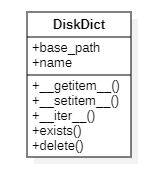
\includegraphics[width=0.25\columnwidth]{immagini/uml-diskdict.jpg} 
    \caption{Diagramma classe DiskDict}
    \label{fig:uml-diskdict}
\end{figure}

La classe \texttt{DiskDict} viene sfruttata per poter accedere e modificare le istanze delle classi, utilizzando la stessa notazione usata per i dizionari in Python. Attraverso l'identificativo utente infatti, la callback interessata può accedere al file in memoria e \texttt{DiskDict} si occuperà del recupero e della ricostruzione dell'oggetto, che viene poi restituito per poter essere utilizzato.


\paragraph{Pulizia dei file inutilizzati}
Il salvataggio dello stato condiviso su disco portava alla creazione di parecchi file. Quando l'utente si disconnette dal sistema, tutti questi file diventano inutili e vanno eliminati, per evitare lo speco di memoria.
\\
Per capire quando un utente si disconnette, il server mantiene una mappa, salvata su disco, che contiene tutti gli identificativi utente attuali con i relativi timestamp. Ad ogni nuova connessione, il nuovo identificativo utente viene aggiunto alla mappa. Questi timestamp sono poi aggiornati periodicamente, a brevi intervalli, da un timer gestito dal client di ogni utente.
\\ 
Dopo un intervallo prefissato di tempo, il server avvia un processo secondario, che ha il compito di comparare i timestamp di tutti gli utenti con il timestamp attuale: se la differenza supera una certa soglia predefinita, l'utente viene considerato disconnesso e tutti i file a lui collegati vengono cancellati. Infine l'identificativo viene rimosso dalla mappa gestita dal server.
\\
Questo semplice sistema funziona perché quando l'utente si disconnette, il timer gestito dal client termina di aggiornare la mappa utenti del server. Ovviamente è necessario aggiustare correttamente i vari intervalli e soglie, e questo è stato fatto tramite osservazione empiriche.


\paragraph{Gestire l'unicità dei nomi degli esperimenti e del caricamento dei process models}
Per rendere univoci i nomi degli esperimenti, che sono salvati dal sistema su disco insieme a tutti i dati generati (process model, raccomandazioni e spiegazioni) si è deciso di aggiungere al nome stesso il timestamp di creazione. Questo risolve il problema e rende univoci i nomi degli esperimenti salvati sul file system del server.
\\
Il nome dell'esperimento però è utilizzato anche per visualizzare i vari process models già allenati, disponibili per essere caricati (vedasi il flusso si esecuzione alternativo descritto nella \autoref{subsec:training}) e, aggiungere il timestamp al nome, può rendere la lettura di quest'ultimo difficile.
Per evitare questo, quando il nome dell'esperimento deve essere mostrato all'utente, questo viene diviso dal timestamp e i due dati vengono visualizzati separatamente (esempio in \autoref{fig:caricamento-modello})
\\ \\
Un ultimo problema individuato riguarda il caricamento dei process models già allenati per saltare la fase di training. Infatti se due utenti selezionano lo stesso process model, questi andranno ad operare sugli stessi file su disco, e l'utente con l'esecuzione che termina per ultima andrà a sovrascrivere i file generati dal primo utente. \\
La soluzione decisa per questo problema è quella di duplicare i file del process model. Quindi, quando un'utente carica un process model già allenato, i file che compongono quest'ultimo vengono duplicati e il nome dell'esperimento viene aggiornato con il nuovo timestamp. Così facendo viene effettivamente creato un nuovo esperimento, l'unicità dei nomi è mantenuta e ogni utente può operare su una copia separata e personale del process model, evitando qualsiasi rischio di sovrascrittura.


 
